% -----------------------------------------------------------------------------
% Metodologia
% -----------------------------------------------------------------------------

\chapter{Metodologia}
\label{chap:metodologia}

A metodologia utilizada na realização desse trabalho consiste em 6 etapas, 
como mostrado na Figura \ref{fig:metodologia}.

\begin{figure}[!htb]
    \centering
    \caption{Metodologia utilizada no trabalho}
    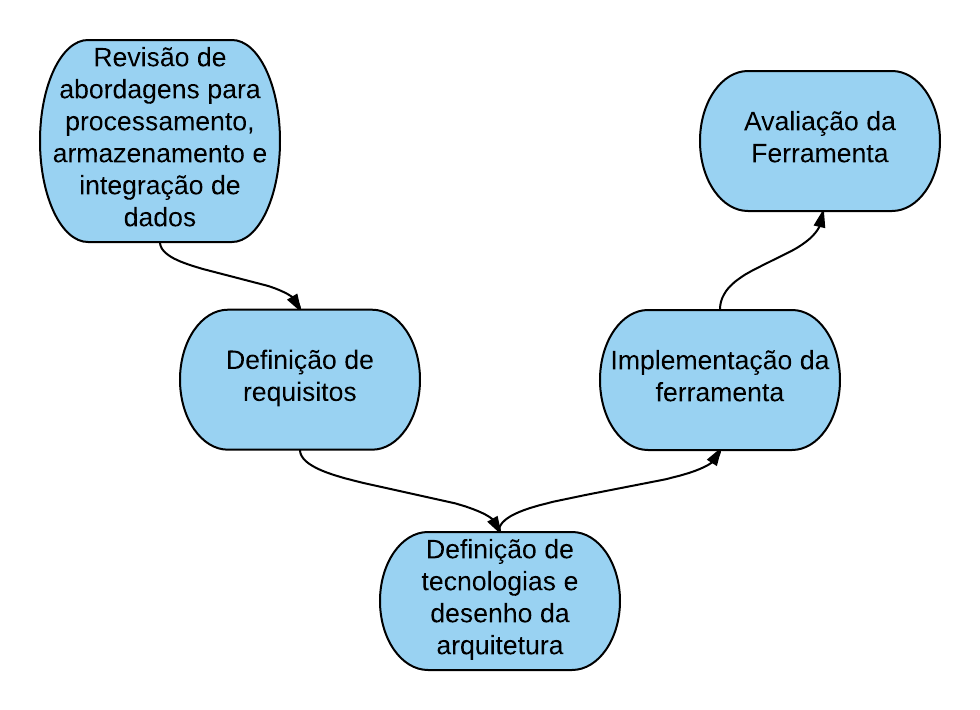
\includegraphics[width=0.8\textwidth]{./04-figuras/metodologia}
    \fonte{O Autor}
    \label{fig:metodologia}
\end{figure}


Como demonstrado na Figura \ref{fig:metodologia}, o primeiro passo da metodologia consistiu em revisar abordagens 
já existentes para o processamento, armazenamento e integração de dados. Essa etapa 
levantou quais as melhores práticas e alternativas a serem aplicadas no contexto dos DGAs. 
Para isso foi realizado a revisão da literatura acerca do tema, o que deu origem ao capitulo 
\ref{chap:trabRelac}.

A segunda etapa consistiu no levantamento dos requisitos funcionais e não funcionais da 
ferramenta, com o objetivo de delimitar o escopo da mesma. Para isso foi realizada uma reunião
com especialistas na área e também foi levado em consideração a revisão da literatura 
feita no passo anterior. Como produto dessa etapa foi gerado um \textit{backlog} com as 
funcionalidades definidas.

A partir dos requisitos levantados anteriormente foram definidas as tecnologias e o desenho 
da arquitetura que possibilitaram o desenvolvimento da ferramenta. Nesse processo se destaca 
a definição do modelo de dados, a forma de acesso e importação dos dados, e quais metadados
serão especificados. Isso foi feito com base na revisão das abordagens realizada no primeiro
passo. Após a definição dos requisitos, das tecnologias e feito o desenho da arquitetura 
foi realizada a implementação da ferramenta. Nesse passo ocorreu a codificação da ferramenta
segundo as tecnologias escolhidas. 

Com o término do desenvolvimento a ferramenta foi avaliada segundo a perspectiva do usuário. 
Essa análise traçou as vantagens e limitações da ferramenta proposta a partir desse 
ponto de vista.
